First, lets go over in a bit more detail what we mean by {\it \bf series}. Two elements are in series if and only if:
\begin{itemize}
\item Those elements share a common node
\item No other elements share the same node
\end{itemize}

% Figure of Resistors in Series
\begin{figure}
%  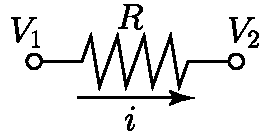
\includegraphics[width=0.5\linewidth]{figures/ohmsLaw}
  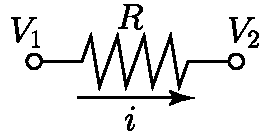
\includegraphics{figures/ohmsLaw}
  \caption{The two resistors above are the only circuit elements connected to node $C$, which means that any current from node $A$ to $C$ will also have to travel from $C$ to $B$.}
  \label{fig:series}
\end{figure}

In this case, there is exactly one path for current to follow through both resistors.  Because of this, we can write the following:
\begin{eqnarray}
  \label{eq:series1} \Delta V_1 &=& V_A-V_C = i R_1 \\ 
  \label{eq:series2} \Delta V_2 &=& V_C-V_B = i R_2 
\end{eqnarray}

Now, our goal is to create simpler circuit which has the same characteristics as seen by nodes $A$ and $B$. The only way to get simpler is to have a single circuit between nodes $A$ and $B$ with a resistance which we still need to determine.

We want our new circuit to have the following characteristics:
\begin{itemize}
\item The current through the new resistor should still be the $i$ that passes through $R_1$ and $R_2$
\item The voltage difference across the new resistor should be $V_A - V_B$
\end{itemize}

We can fulfill those two requirements by summing equations \ref{eq:series1} and \ref{eq:series2}:
\begin{equation} \label{eq:series3}
\Delta V_1 + \Delta V_2 = V_A - V_B = i (R_1 + R_2)
\end{equation}

Equation \ref{eq:series3} essentially states that we can replace both resistors with a single resistor that has a resistance
\begin{equation} \label{eq:seriesEquivalent}
R_{EQ}=R_1+R_2.
\end{equation}
